\documentclass[aspectratio=169,11pt]{beamer}

\usepackage[utf8]{inputenc}
\usepackage[T1]{fontenc}
\usepackage{graphicx}
\usepackage{booktabs}
\usepackage{array}
\usepackage{xcolor}
\usepackage{hyperref}

\usetheme{Madrid}
\usecolortheme{default}
\setbeamertemplate{navigation symbols}{}
\setbeamertemplate{footline}[frame number]
\setbeamercolor{structure}{fg=black}
\setbeamercolor{frametitle}{fg=black,bg=gray!10}
\setbeamercolor{title}{fg=black}
\setbeamersize{text margin left=8mm,text margin right=8mm}

\definecolor{railblue}{HTML}{2F5D8C}
\definecolor{railgreen}{HTML}{3A7D44}
\definecolor{railorange}{HTML}{A55A20}
\definecolor{railgray}{HTML}{F2F2F2}

\newcommand{\smallsource}[1]{\par\vspace{1mm}{\tiny\raggedright Fuente: #1\par}}
\newcommand{\imagecaption}[1]{\par\vspace{1mm}{\small\bfseries #1\par}}
\newcommand{\tightlist}{\setlength{\itemsep}{2pt}\setlength{\parskip}{0pt}}
\newcommand{\blockbox}[2]{%
  \fcolorbox{black!45}{gray!8}{\parbox[c][18mm][c]{\dimexpr#1-2\fboxsep-2\fboxrule\relax}{\centering\footnotesize #2}}%
}

\title[AudioLab]{AudioLab}
\subtitle{Plataforma USB de audio y DSP embebido}
\author{Martín Ramírez Espinosa}
\institute{maramirezes@unal.edu.co}
\date{4 de junio de 2026}

\begin{document}

\begin{frame}[plain]
  \vspace{12mm}
  \begin{center}
    {\fontsize{30}{34}\selectfont\bfseries AudioLab}

    \vspace{5mm}
    {\Large Plataforma USB de audio y DSP embebido}

    \vspace{12mm}
    {\large Martín Ramírez Espinosa}

    \vspace{2mm}
    {\normalsize maramirezes@unal.edu.co}

    \vspace{8mm}
    {\normalsize 4 de junio de 2026}

    \vspace{8mm}
    {\small Tarjeta hija para NUCLEO-F429ZI basada en el codec estéreo TLV320AIC3104.}
  \end{center}
\end{frame}

\begin{frame}{Intención del Proyecto}
  \begin{columns}[T,totalwidth=\textwidth]
    \begin{column}{0.56\textwidth}
      \textbf{AudioLab} busca convertir una NUCLEO-F429ZI en una plataforma de laboratorio para audio USB, adquisición/reproducción estéreo y procesamiento digital en tiempo real.

      \vspace{2mm}
      \begin{itemize}\tightlist
        \item Usuarios objetivo: cursos, laboratorios de señales, prototipos de audio y validación de DSP embebido.
        \item Función principal: transportar audio entre un PC, el STM32F429ZI y un codec TLV320AIC3104.
        \item Comportamiento esperado: reproducir, capturar y eventualmente procesar audio a 48 kHz con diagnóstico de fallas.
      \end{itemize}
    \end{column}
    \begin{column}{0.40\textwidth}
      \centering
      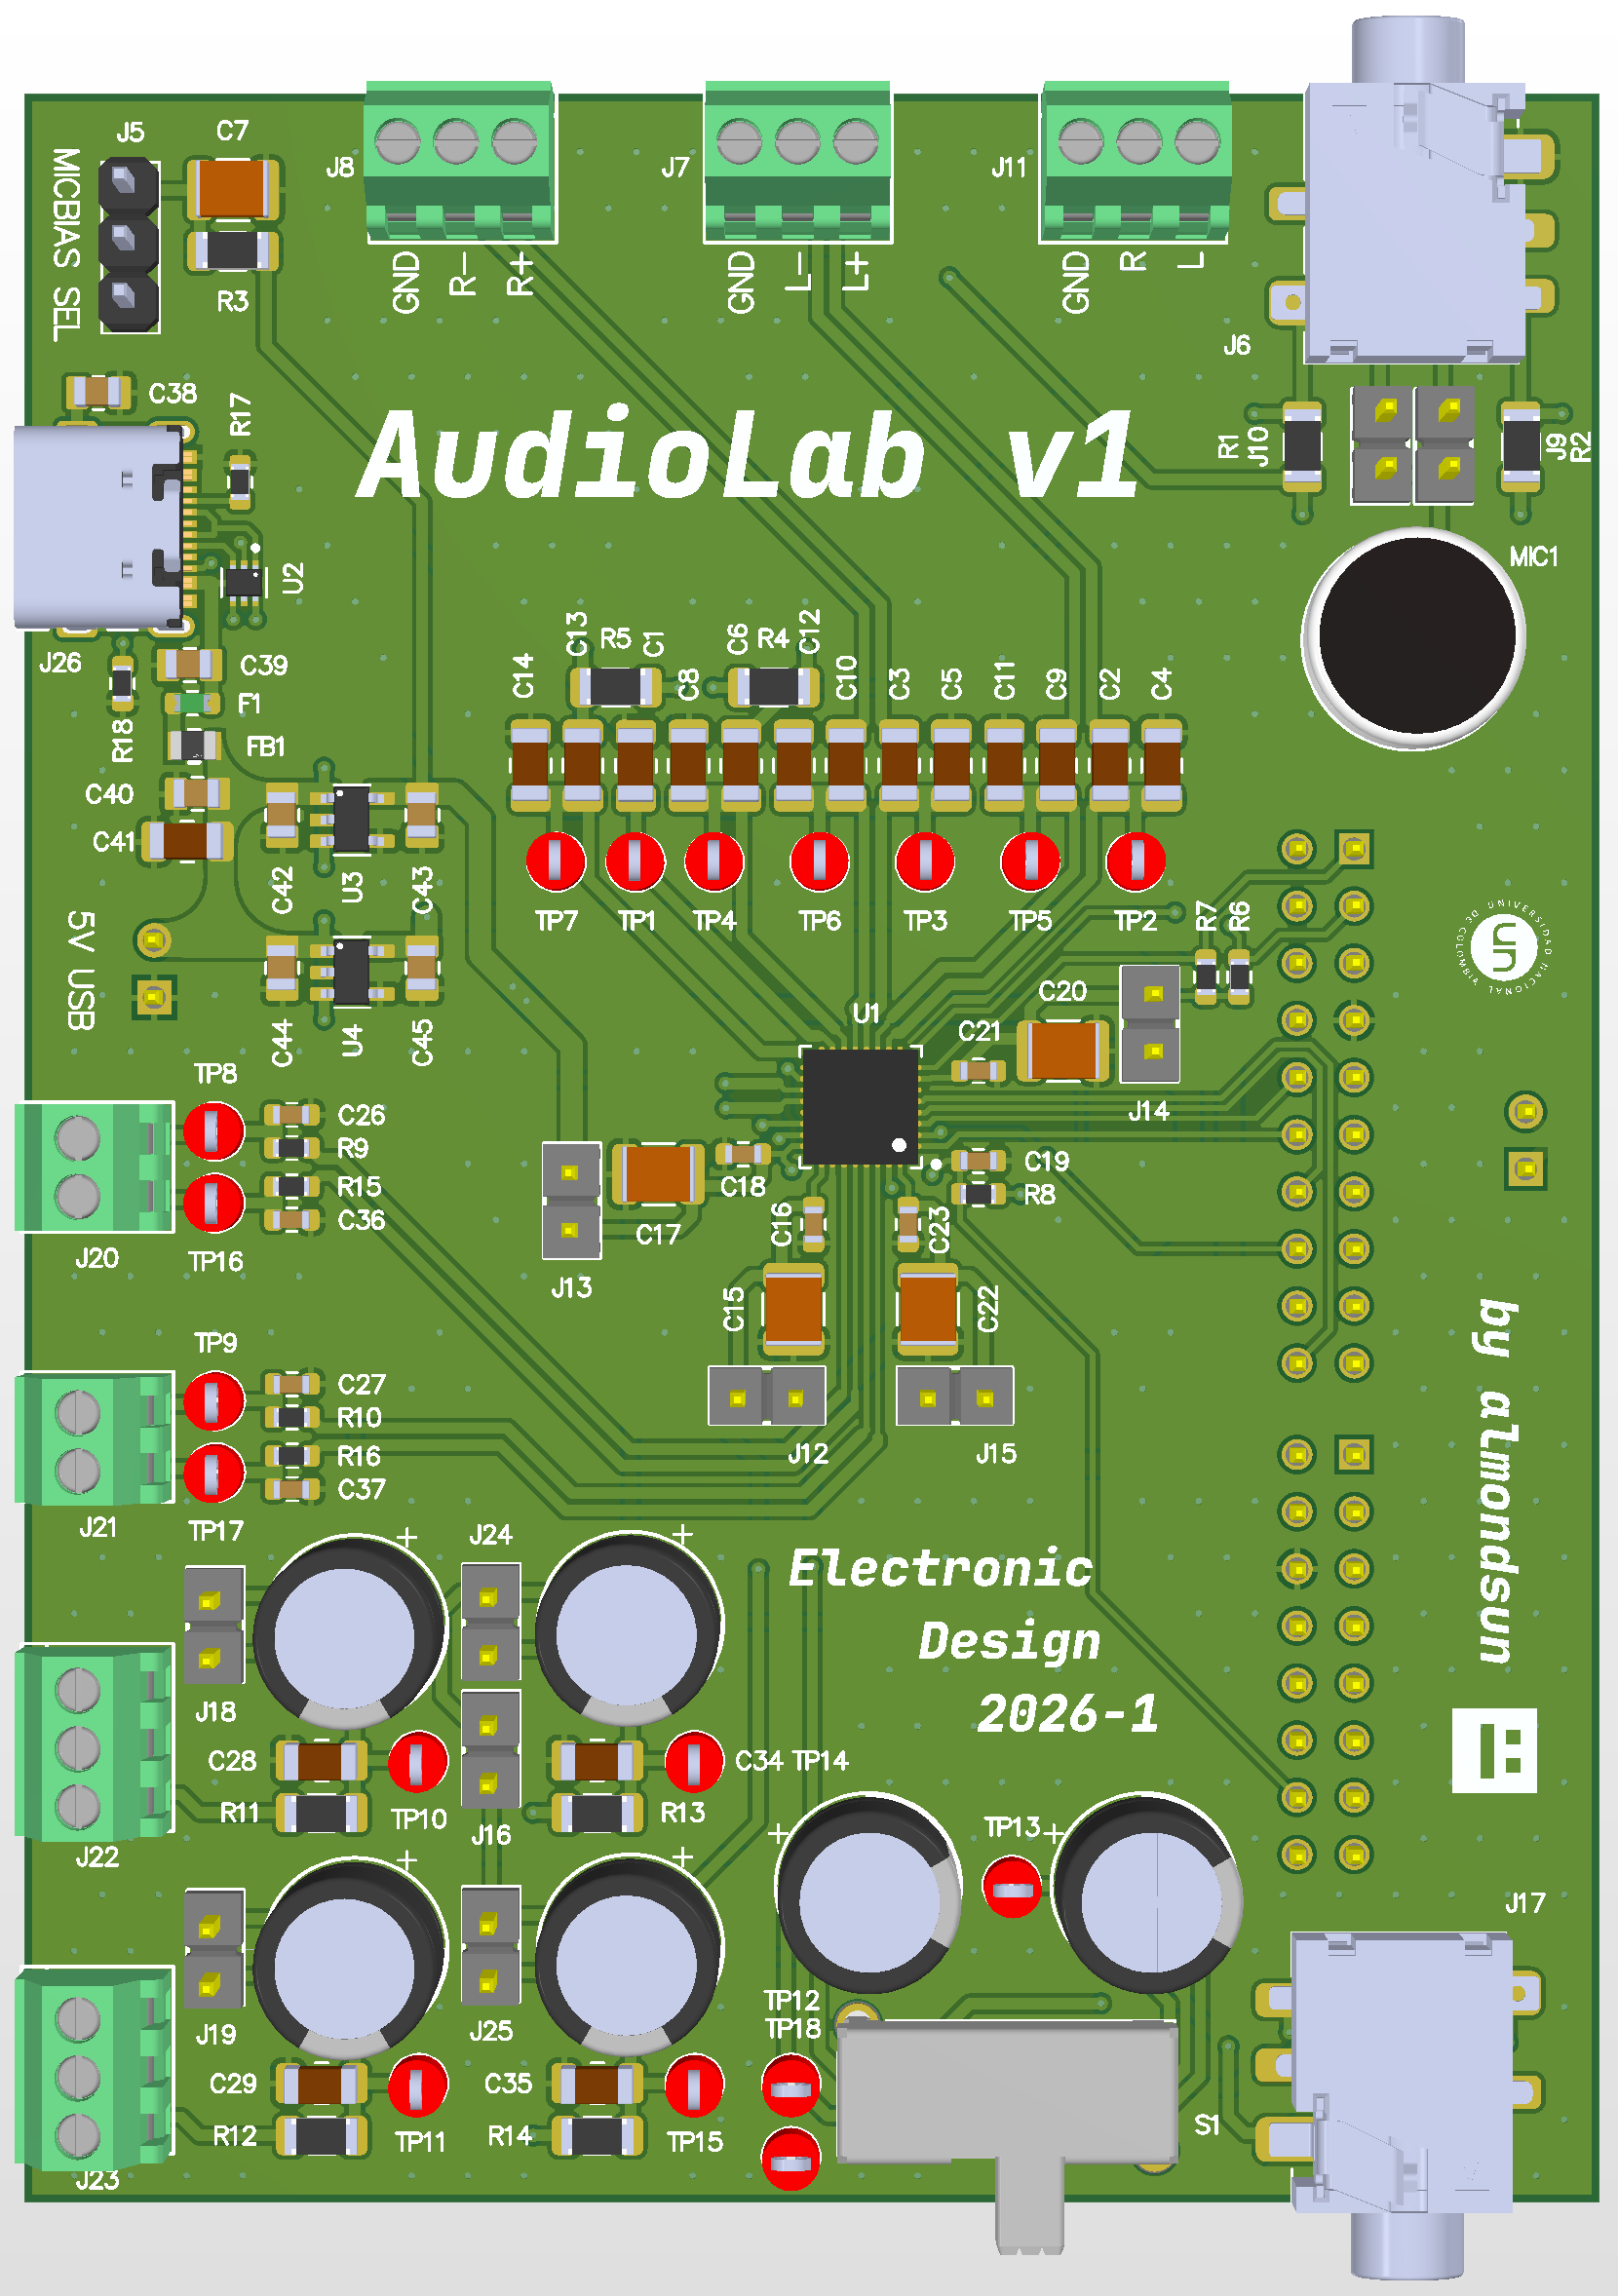
\includegraphics[height=0.66\textheight]{../../../assets/AudioLab-above.png}
      \smallsource{\texttt{assets/AudioLab-above.png}}
    \end{column}
  \end{columns}
\end{frame}

\begin{frame}{Arquitectura de Bloques}
  \centering
  \begin{tabular}{>{\centering\arraybackslash}m{0.20\textwidth} c >{\centering\arraybackslash}m{0.25\textwidth} c >{\centering\arraybackslash}m{0.25\textwidth}}
    \blockbox{\linewidth}{\textbf{Computador}\\audio USB\\control y diagnóstico} &
    $\Longleftrightarrow$ &
    \blockbox{\linewidth}{\textbf{NUCLEO-F429ZI}\\dispositivo USB\\maestro SAI/I2S\\control I2C\\DSP en firmware} &
    $\Longleftrightarrow$ &
    \blockbox{\linewidth}{\textbf{AudioLab}\\TLV320AIC3104\\ADC/DAC\\entradas/salidas analógicas}
  \end{tabular}

  \vspace{5mm}
  \begin{columns}[T,totalwidth=\textwidth]
    \begin{column}{0.32\textwidth}
      \textbf{Control}
      \begin{itemize}\tightlist
        \item I2C para registros del codec.
        \item Reset seguro del TLV320AIC3104.
      \end{itemize}
    \end{column}
    \begin{column}{0.32\textwidth}
      \textbf{Audio digital}
      \begin{itemize}\tightlist
        \item STM32 como maestro SAI/I2S.
        \item MCLK, BCLK, WCLK, DIN y DOUT.
      \end{itemize}
    \end{column}
    \begin{column}{0.32\textwidth}
      \textbf{Audio analógico}
      \begin{itemize}\tightlist
        \item Entradas para línea/micrófono.
        \item Salidas para audífonos/línea y medición.
      \end{itemize}
    \end{column}
  \end{columns}
  \smallsource{\texttt{docs/specs/system/requirements.md} y \texttt{docs/specs/hardware/architecture.md}}
\end{frame}

\begin{frame}{Árbol de Potencia}
  \scriptsize
  \centering
  \begin{tabular}{>{\centering\arraybackslash}m{0.24\textwidth}}
    \colorbox{railgray}{\parbox{0.22\textwidth}{\centering \textbf{USB-C / VBUS}\\entrada de potencia}}
  \end{tabular}

  \vspace{1mm}
  $\Downarrow$

  \vspace{1mm}
  \begin{tabular}{>{\centering\arraybackslash}m{0.24\textwidth}}
    \colorbox{railgray}{\parbox{0.22\textwidth}{\centering \textbf{5V}\\fusible, filtro y desacople}}
  \end{tabular}

  \vspace{1mm}
  $\Downarrow$

  \vspace{1mm}
  \begin{tabular}{>{\centering\arraybackslash}m{0.26\textwidth} >{\centering\arraybackslash}m{0.26\textwidth} >{\centering\arraybackslash}m{0.26\textwidth}}
    \colorbox{railblue!15}{\parbox{0.24\textwidth}{\centering \textbf{3V3}\\AVDD, DRVDD\\IOVDD}} &
    \colorbox{railgreen!15}{\parbox{0.24\textwidth}{\centering \textbf{1V8}\\DVDD\\núcleo digital}} &
    \colorbox{railorange!15}{\parbox{0.24\textwidth}{\centering \textbf{Señales USB}\\USB\_D\_P\\USB\_D\_N}}
  \end{tabular}

  \vspace{2mm}
  \begin{itemize}\tightlist
    \item La hoja \texttt{PowerSupply.SchDoc} implementa entrada USB-C, protección ESD, filtrado y desacople sobre VBUS/5V.
    \item TLV75533 genera 3V3 para AVDD, DRVDD e IOVDD; TLV70018 genera 1V8 para DVDD.
    \item Las líneas USB\_D\_P y USB\_D\_N pasan por protección ESD antes de llegar al sistema.
  \end{itemize}
  \smallsource{\texttt{hardware/docs/schematics.pdf}, hoja \texttt{PowerSupply.SchDoc}}
\end{frame}

\begin{frame}{Prueba de Concepto}
  \footnotesize
  \begin{columns}[T,totalwidth=\textwidth]
    \begin{column}{0.48\textwidth}
      \textbf{Evidencia disponible}
      \begin{itemize}\tightlist
        \item Firmware PlatformIO para NUCLEO-F429ZI con estructura de estado, control de bus, diagnósticos y pruebas unitarias.
        \item Prototipo DSPLink como evidencia de arquitectura STM32, no como contrato final de AudioLab.
        \item Prototipo de interfaz host asignado a \texttt{software/host/ui-prototypes/}.
      \end{itemize}
    \end{column}
    \begin{column}{0.48\textwidth}
      \textbf{Límite técnico}
      \begin{itemize}\tightlist
        \item DSPLink controla ADAU1701/TSA1701; AudioLab requiere control TLV320AIC3104.
        \item En AudioLab el procesamiento en tiempo real pertenece al STM32F429ZI.
        \item Trabajo pendiente: migrar el firmware a audio USB, SAI/I2S y controlador TLV320AIC3104.
      \end{itemize}
    \end{column}
  \end{columns}

  \vspace{4mm}
  \centering
  \blockbox{0.82\textwidth}{La prueba de concepto validó disciplina de estados, comunicación embebida, diagnósticos y organización de firmware; el siguiente paso es reemplazar las suposiciones DSPLink por el contrato TLV320AIC3104.}
  \smallsource{\texttt{dsplink-allocation.md} y \texttt{firmware/stm32/}}
\end{frame}

\begin{frame}{Esquemático: Sistema}
  \begin{columns}[T,totalwidth=\textwidth]
    \begin{column}{0.58\textwidth}
      \centering
      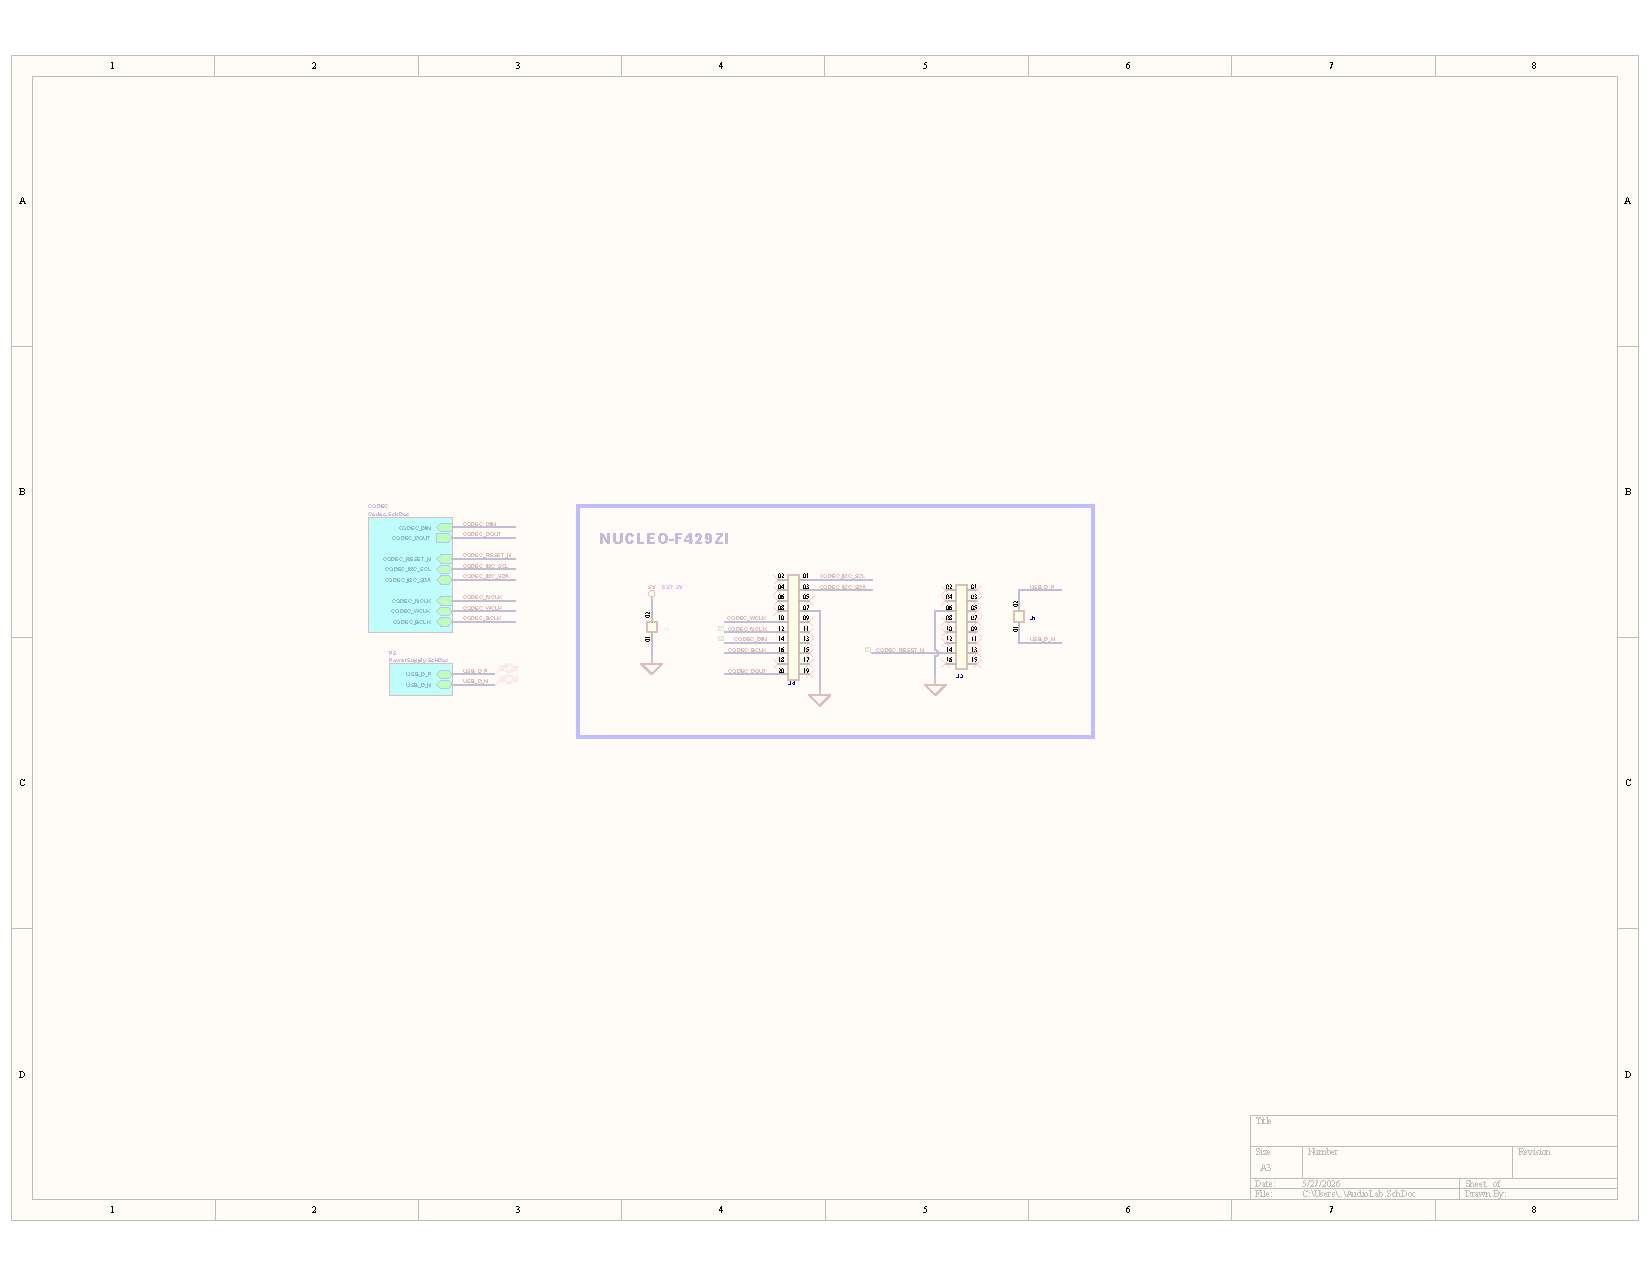
\includegraphics[page=1,width=\linewidth]{../../../hardware/docs/schematics.pdf}
    \end{column}
    \begin{column}{0.38\textwidth}
      \textbf{Decisiones visibles}
      \begin{itemize}\tightlist
        \item Hojas jerárquicas separadas: \texttt{CODEC} y \texttt{PS}.
        \item Nets explícitas para I2C, reset, USB y audio digital.
        \item Conexión a NUCLEO-F429ZI mediante encabezados.
        \item Separación entre la tarjeta codec y la placa controladora.
      \end{itemize}
      \smallsource{\texttt{hardware/docs/schematics.pdf}, pág. 1}
    \end{column}
  \end{columns}
\end{frame}

\begin{frame}{Esquemático: Codec y Alimentación}
  \footnotesize
  \begin{columns}[T,totalwidth=\textwidth]
    \begin{column}{0.48\textwidth}
      \centering
      \includegraphics[page=2,height=0.44\textheight,width=\linewidth,keepaspectratio]{../../../hardware/docs/schematics.pdf}
      \imagecaption{TLV320AIC3104 y rutas de audio}
    \end{column}
    \begin{column}{0.48\textwidth}
      \centering
      \includegraphics[page=3,height=0.44\textheight,width=\linewidth,keepaspectratio]{../../../hardware/docs/schematics.pdf}
      \imagecaption{Regulación y distribución de potencia}
    \end{column}
  \end{columns}

  \vspace{1mm}
  \begin{itemize}\tightlist
    \item El codec concentra conversión ADC/DAC, interfaz I2C, bus SAI/I2S y redes analógicas.
    \item La hoja de potencia documenta el paso de VBUS/5V a 3V3 y 1V8 para los dominios del codec.
  \end{itemize}
  \smallsource{\texttt{hardware/docs/schematics.pdf}, págs. 2--3}
\end{frame}

\begin{frame}{PCB}
  \footnotesize
  \begin{columns}[T,totalwidth=\textwidth]
    \begin{column}{0.58\textwidth}
      \centering
      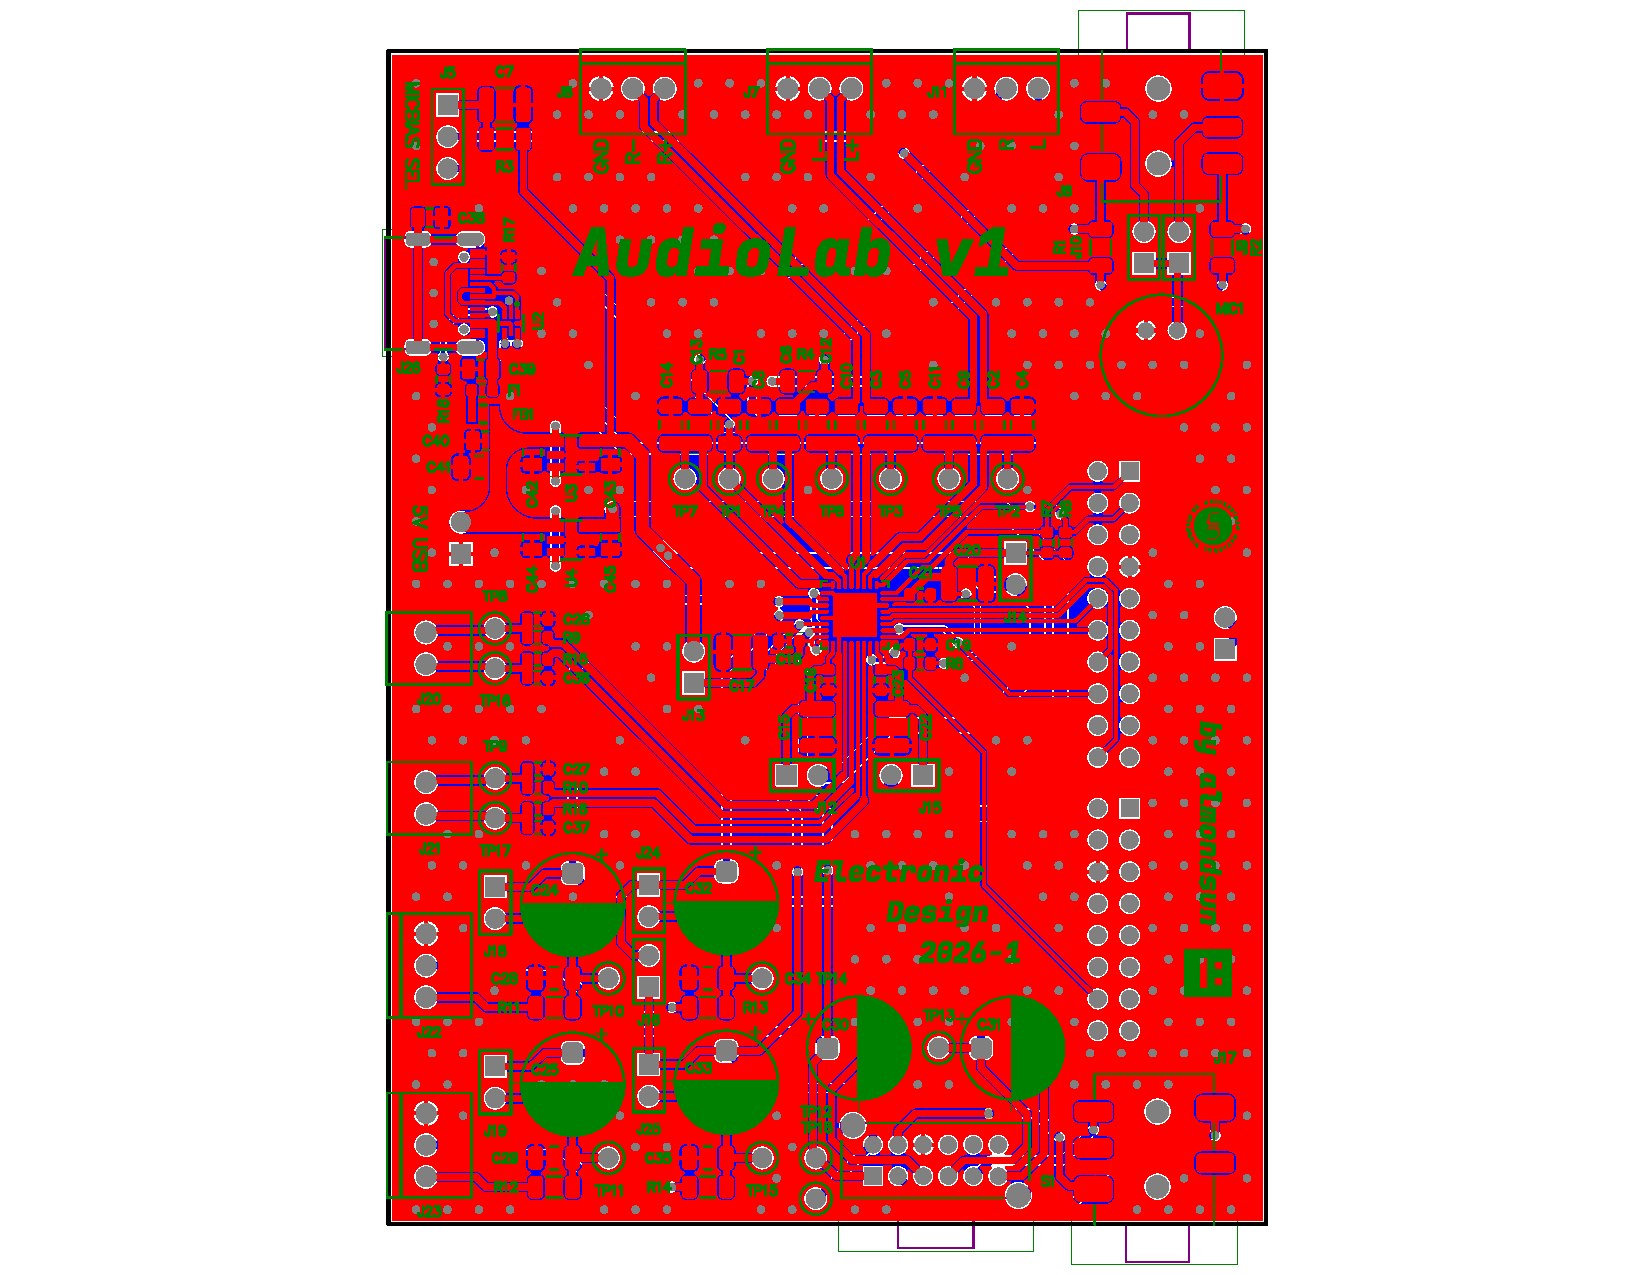
\includegraphics[width=\linewidth]{../../../hardware/docs/pcb.pdf}
    \end{column}
    \begin{column}{0.38\textwidth}
      \textbf{Criterios de construcción}
      \begin{itemize}\tightlist
        \item Organización por bloques: conectores Nucleo, codec, audio analógico, potencia y medición.
        \item Señales de reloj y datos cortas e inspeccionables.
        \item Acceso de laboratorio para rieles, reset, I2C y señales de audio.
        \item Diseño revisado con DRC de Altium: 0 violaciones detectadas.
      \end{itemize}
      \smallsource{\texttt{hardware/docs/pcb.pdf} y DRC de Altium}
    \end{column}
  \end{columns}
\end{frame}

\begin{frame}{Render 3D}
  \begin{columns}[T,totalwidth=\textwidth]
    \begin{column}{0.48\textwidth}
      \centering
      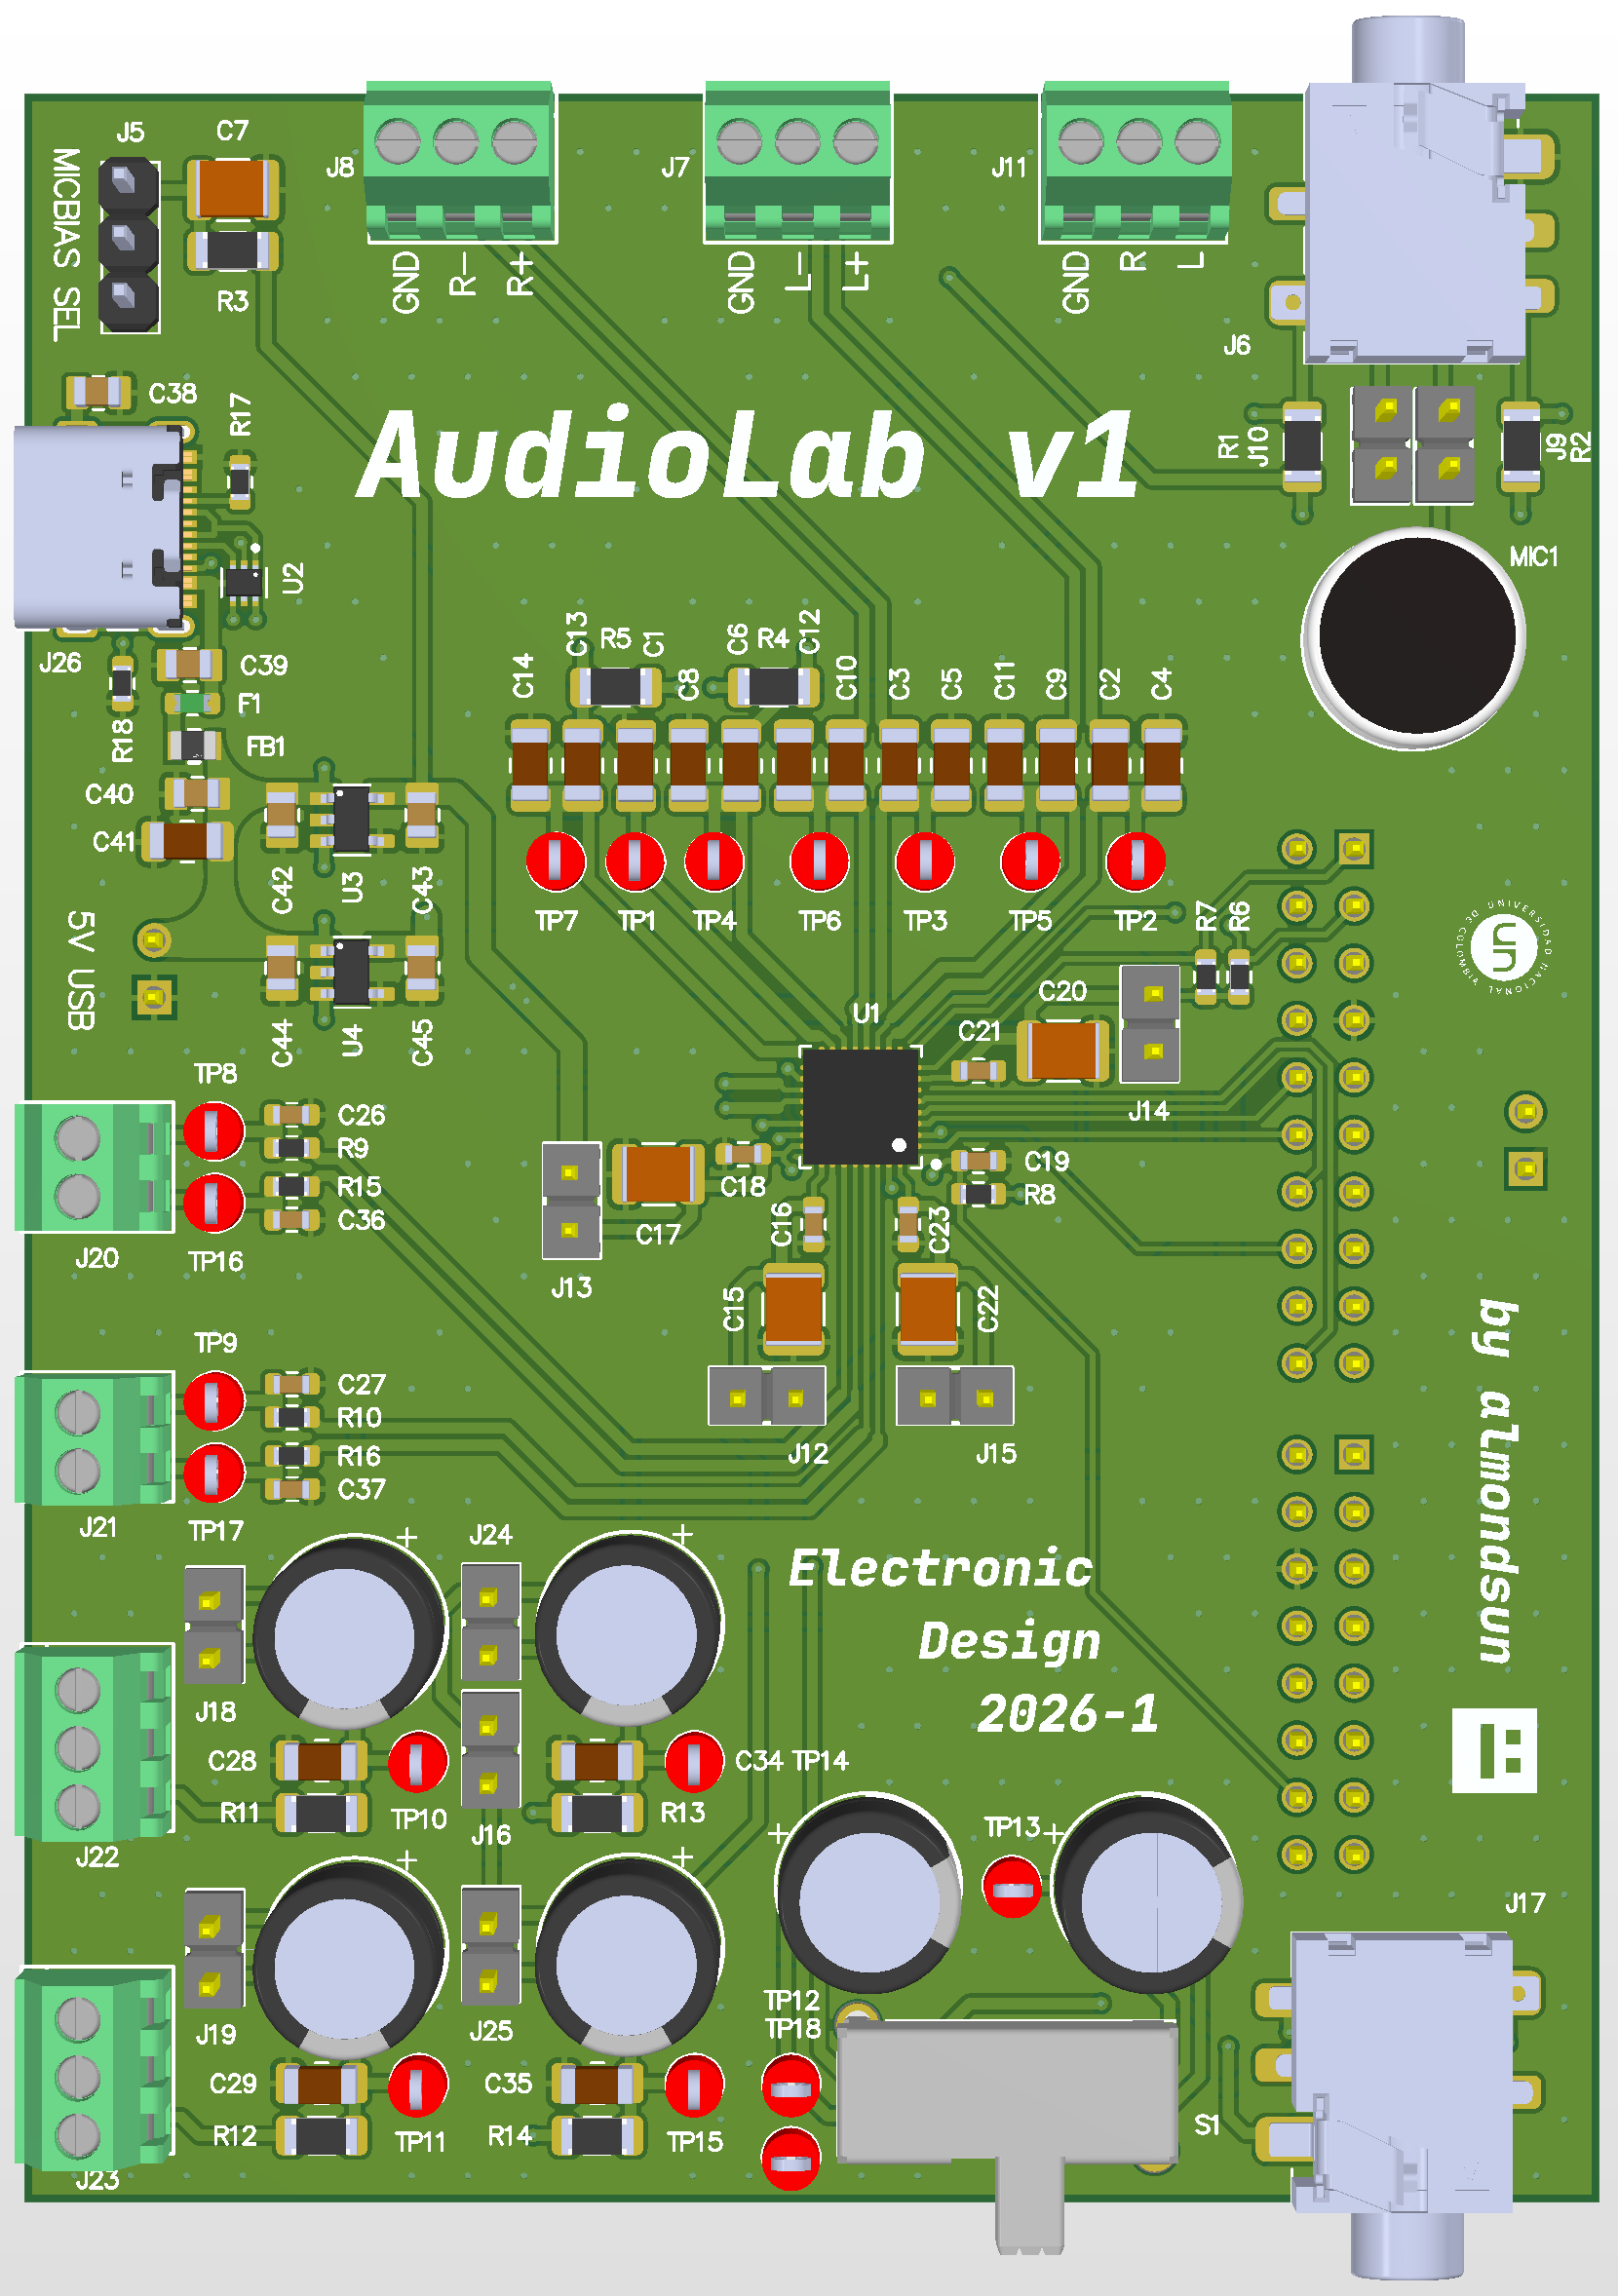
\includegraphics[height=0.68\textheight]{../../../assets/AudioLab-above.png}
      \imagecaption{Vista superior}
    \end{column}
    \begin{column}{0.48\textwidth}
      \centering
      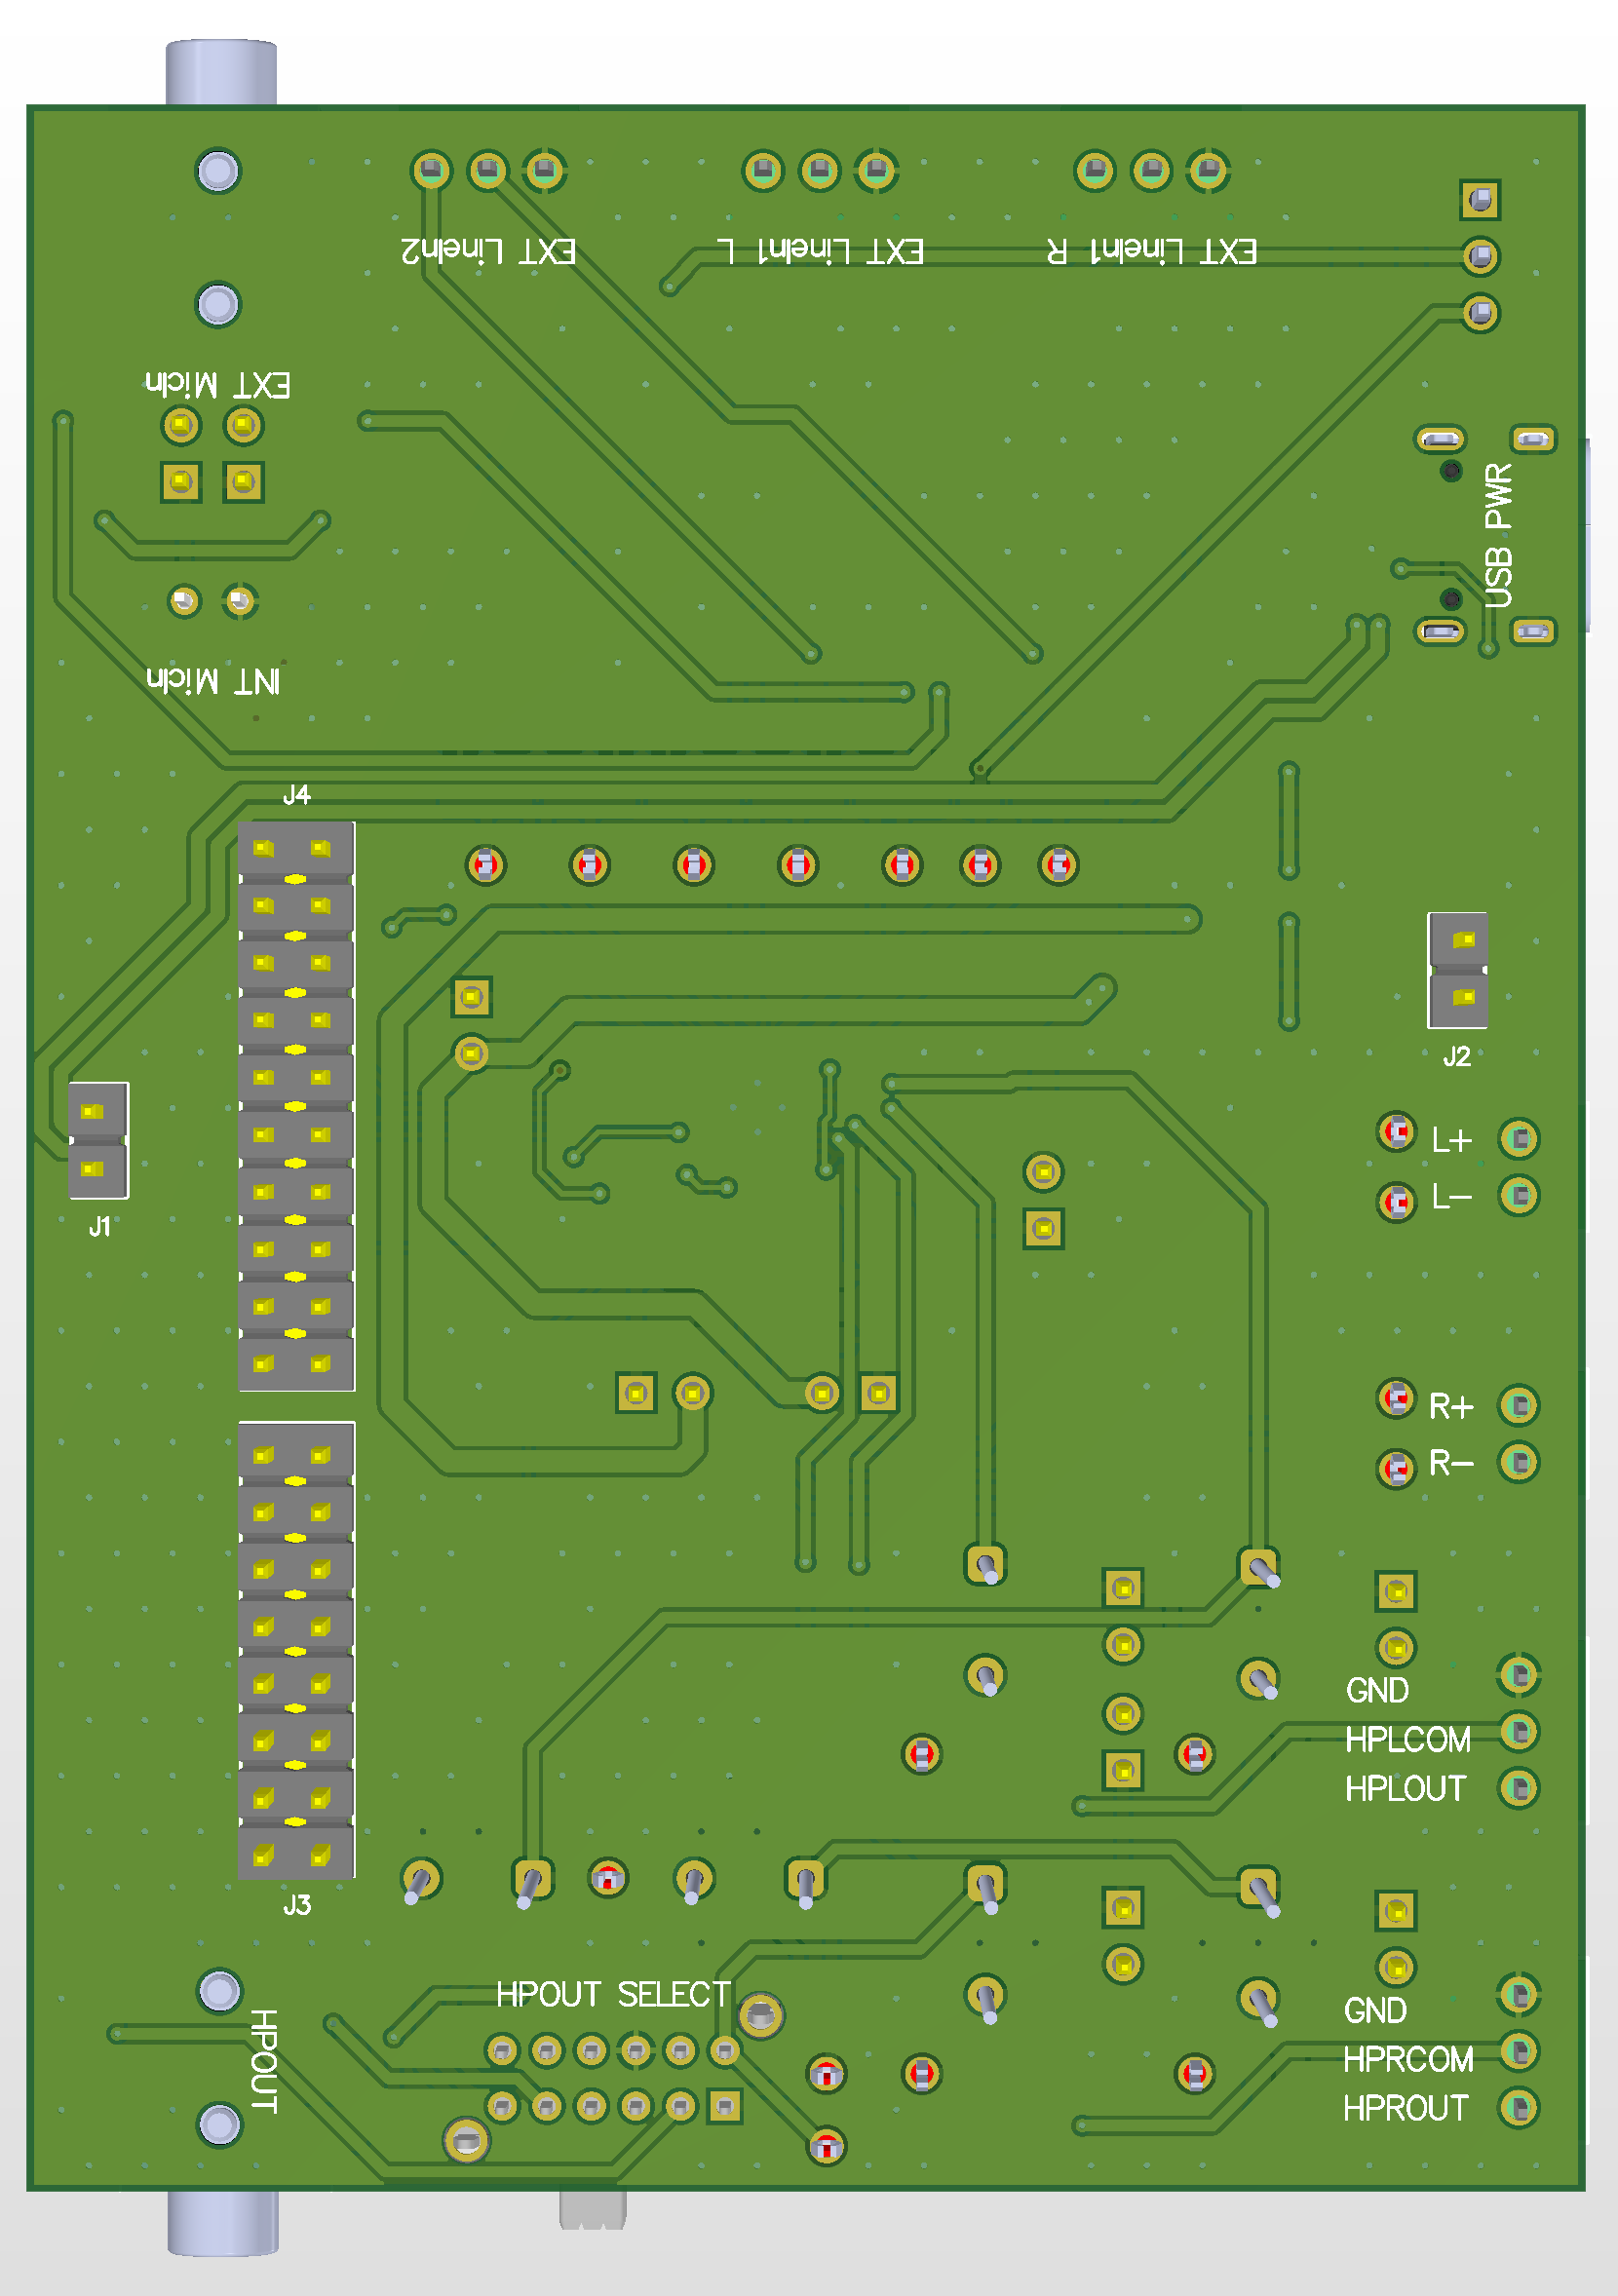
\includegraphics[height=0.68\textheight]{../../../assets/AudioLab-below.png}
      \imagecaption{Vista inferior}
    \end{column}
  \end{columns}
  \smallsource{\texttt{assets/AudioLab-above.png} y \texttt{assets/AudioLab-below.png}}
\end{frame}

\begin{frame}{Estado Actual y Próximos Pasos}
  \begin{columns}[T,totalwidth=\textwidth]
    \begin{column}{0.48\textwidth}
      \textbf{Avances consolidados}
      \begin{itemize}\tightlist
        \item Contrato de hardware TLV320AIC3104 documentado.
        \item Esquemático, PCB, archivos Gerber, taladros y DRC exportados.
        \item Separación clara entre hardware final y prueba de concepto DSPLink.
      \end{itemize}
    \end{column}
    \begin{column}{0.48\textwidth}
      \textbf{Trabajo pendiente}
      \begin{itemize}\tightlist
        \item Migrar firmware a codec TLV320AIC3104, SAI/I2S, USB Audio y DSP STM32.
        \item Fabricar/ensamblar PCB y medir rieles antes de activar audio.
        \item Registrar prueba de lazo, latencia, corriente y fallas de búfer.
      \end{itemize}
    \end{column}
  \end{columns}

  \vspace{4mm}
  \blockbox{0.90\textwidth}{Conclusión técnica: una tarjeta de audio requiere contrato de potencia, secuencia de reset, medición de rieles, control de codec y evidencia de audio digital/analógico trabajando en conjunto.}
\end{frame}

\begin{frame}{Plan de Validación}
  \begin{columns}[T,totalwidth=\textwidth]
    \begin{column}{0.48\textwidth}
      \textbf{Antes de energizar}
      \begin{itemize}\tightlist
        \item Inspección visual y continuidad contra cortos.
        \item Alimentación con corriente limitada.
        \item Medición de VBUS, 5V, 3V3 y 1V8.
        \item Confirmar reset seguro del codec.
      \end{itemize}
    \end{column}
    \begin{column}{0.48\textwidth}
      \textbf{Puesta en marcha funcional}
      \begin{itemize}\tightlist
        \item Comunicación I2C con TLV320AIC3104.
        \item Relojes MCLK, BCLK y WCLK.
        \item Reproducción, captura y prueba de lazo.
        \item Medición de corriente, ruido básico y eventos de subdesbordamiento o sobredesbordamiento.
      \end{itemize}
    \end{column}
  \end{columns}
  \smallsource{\texttt{docs/specs/hardware/architecture.md} y \texttt{docs/specs/power/architecture.md}}
\end{frame}

\begin{frame}{Referencias}
  \scriptsize
  \begin{itemize}\tightlist
    \item Texas Instruments, \textit{TLV320AIC3104 Stereo Audio Codec}, hoja de datos local: \texttt{hardware/references/tlv320aic3104.pdf}.
    \item STMicroelectronics, \textit{NUCLEO-F429ZI / Nucleo-144 user manual}, referencia local bajo \texttt{hardware/references/}.
    \item STMicroelectronics, documentación STM32F429ZI y placa Nucleo: \texttt{hardware/references/nucleo-f429zi.pdf}.
    \item Texas Instruments, reguladores TLV700 y TLV755P: \texttt{hardware/references/tlv700.pdf}, \texttt{hardware/references/tlv755p.pdf}.
    \item Repositorio AudioLab: \texttt{README.md}, \texttt{docs/specs/system/requirements.md}, \texttt{docs/specs/hardware/architecture.md}, \texttt{docs/specs/power/architecture.md}.
    \item Evidencia de diseño: \texttt{hardware/docs/schematics.pdf}, \texttt{hardware/docs/pcb.pdf}, \texttt{hardware/altium/project/Project Outputs for AudioLab/}.
  \end{itemize}
\end{frame}

\end{document}
